\documentclass{article}
\usepackage[utf8]{inputenc}

\title{100 Ideias}
%\numberofauthors{4} %  in this sample file, there are a *total*
% of EIGHT authors. SIX appear on the 'first-page' (for formatting
% reasons) and the remaining two appear in the \additionalauthors section.
%
\author{
% You can go ahead and credit any number of authors here,
% e.g. one 'row of three' or two rows (consisting of one row of three
% and a second row of one, two or three).
%
% The command \alignauthor (no curly braces needed) should
% precede each author name, affiliation/snail-mail address and
% e-mail address. Additionally, tag each line of
% affiliation/address with \affaddr, and tag the
% e-mail address with \email.
%
% 1st. author
\alignauthor
André Carvalho\\
       \affaddr{FCUP - DCC}\\
       \affaddr{Motivation Coach}\\
       \affaddr{Documenter}\\
\and
% 2nd. author
\alignauthor
André Fonseca\\
       \affaddr{FCUP - DCC}\\
       \affaddr{Task Master}\\
       \affaddr{Developer}\\
\and
% 3rd. author
\alignauthor Bruno Cabral\\
       \affaddr{FCUP - DCC}\\
       \affaddr{Resources Support}\\
       \affaddr{Researcher}\\
\and  % use '\and' if you need 'another row' of author names
% 4th. author
\alignauthor Tiago Castanheira\\
       \affaddr{FCUP - DCC}\\
       \affaddr{Mediator}\\
       \affaddr{Architect}\\
}




\date{April}

\usepackage{natbib}
\usepackage{graphicx}

\begin{document}
%\keywords{Helping\\ Caring \\ Integration}
\maketitle
\begin{abstract}
    Este relatorio olha para o trabalho que temos vindo a realizar durante o semestre. O objectivo deste  trabalho é ajudar os refugiados possibilitando uma plataforma web que os ajude a decidir sobre qual distrito do Pais no qual querem viver.Observamos que muitas destas pessoas não conhecem as culturas para a qual vão ser inseridas, e por esta razão decidimos facilitar a integração dos proprios na comunidade onde vão ser colocados.\\Esperamos que a nossa contribuição ajude os refugiados a perceber melhor e a facilitar a sua integração na comunidade portuguesa e que permitirá uma melhor consideração individual sobre estes individuos.
    
    
\end{abstract}
\section{Introdução}

%% The ``\copyrightspace'' command must be the first command after the
%% start of the first section of the body of your paper. It ensures the
%% copyright space is left at the bottom of the first column on the first
%% page of your paper.

%% \copyrightspace

    Está em curso a maior crise de refugiados desde a IIº Guerra, situação de uma enorme complexidade, para a qual não existe uma resposta simples, nem uma solução isenta de riscos/efeitos perversos.\\Portugal está por enquanto afastado do centro do problema, podendo ter a tentação de o “ignorar“. Deve ser, no entanto, solidário com os restantes países europeus na gestão desta crise humanitária.

\begin{itemize}
    \item Sensibilização e integração: Assim perante este contexto, esperamos que com a criação deste projecto consigamos sensibilizar Portugal para as questões dos direitos de refugiados e ao mesmo tempo ajudar estes na sua integração na comunidade Portuguesa com o envolvimento das instituiçoes locais.
    \item Plataforma de apoio: Dado esta situação esta a ser desenvolvido uma plataforma que promove o apoio aos refugiados na sociadade Portugesa, acolhimento e integração tendo em vista a autonomia e integração dos adultos no mercado de trabalho e das crianças na escola.A plataforma contem também informação cultural e social de cada distrito do pais. 
    \item Missão: Há a noção da urgência da ação humanitária, que pede uma resposta imediata de acolhimento, sem ignorar as intervenções com impacto a médio-longo prazo, como a estabilização política, económica e social das zonas de crise.\\Coloca-se o desafio de uma resposta  solidária e eficaz que evite os egoísmos nacionais, que não aumente a xenofobia e que seja útil.\\Existem instituições da sociedade civil com vontade, disponibilidade e experiência no acolhimento de refugiados que, através de uma plataforma web e através de um modelo colaborativo e articulado, poderiam dar um contributo para este desafio, em complementaridade com a ação do Estado Portugues. 


\end{itemize}

\section{Motivação}
O projecto surgiu da necessidade de tentar sensibilizar
Portugal para a crise humanitaria de refugiados, e ao mesmo
tempo oferecer ajuda na integração destes na comunidade.
Queremos promover uma cultura de acolhimento qualificado
e sustentavel. Queremos elucidar como a sua migração e
efectuada, bem como a falta de condições a que a maior
parte destas pessoas estãoo sujeitas, sejam elas condições alimentares,
higienicas ou financeiras visto que muitas das pessoas
que são recebidas no nosso paiss não estão acostumadas
a maneira de ser, a linngua portuguesa, a comunidade residente,
e o acumular de todos estes factores pode contribuir
para uma exclusao social. Estas pessoas enfrentam tambem
o risco de perseguição, violência de genero e descriminação
religiosa e por vezes racial.
Dito isto temos como missão criar uma plataforma web de
integração de familias para refugiados.
\section{COMO AJUDAR?}
Pensamos que a melhor maneira de ajudar os imigrantes
que escolhem ser parte deste pais e ajuda-los a comprender
melhor os costumes tradicionais e ao mesmo tempo ajuda-los
a fazer parte da comunidade, nos consideramos que a melhor
maneira de passar toda esta informação seria atraves do uso
de um site, criado por nos que contem informação cultural
sobre cada distrito, sociadades civis que estejam dispostos
a ajudar e ONG's. Disponibilizar tambem informação de
como a comunidade Portuguesa pode contribuir para ajudar
esta crise humanitaria.

\section{OBJECTIVOS}
Com este projecto esperamos facilitar a assimilação dos
refugiados no nosso pais, disponibilizando o maximo de informacão relevante sobre Portugal de uma forma simples e
acessivel a todos. O uso do site é tambem perfeito pois e simples
de fazer e tem um custo de manutenção relativamente
baixo, tornando-se assim a melhor maneira de divulgar esta
informacão ao maior numero de pessoas possiveis.
Após conclusão de um pequeno estudo paraa escolha da tecnologia/framework que será trabalhada, induzimos estes objetivos a serem alcançados:
\begin{itemize}
\item Criar uma imagem de sistema para explicar como é que as funcionalidades se interligam e como se usam;
\item Desenvolver a interface web que resolva os problemas identificados
\item Input fácil, leitura rápida
\end{itemize}

\section{BackGround}
Com este projecto em mente para colocar o website online
precisariamos de um dominio e servidor, visto que é apenas
uma ideia inicial o nosso website apenas existe offine.
Não e preciso a utilização de nenhuma tecnologia visto que
basta um editor de texto e browser. Entretanto utilizamos uma JS framework com o nome Bootstrap que contem varios templates 
pre definidos na internet.

\section{OVERVIEW}
O nosso projecto e um website, portanto para iniciar este
projecto e util ter conhecimentos em html, javascript e css.
HTML significa Hyper Text Markup Language, é uma linguagem de marcação basicamente um conjunto de tags de marcação
,todos documentos HTML são descritos por tags HTML,cada tag HTML descreve o conteúdo do documento de maneira diferente.\\
JavaScript é a linguagem de programação HTML e da Web ,juntamente com HTML e CSS , é uma das três principais tecnologias que compoem a internet.
CSS é uma linguagem de estilo que descreve a apresentação de um documento HTML.CSS descreve como elementos devem ser processados no ecra , no papel, ou em outros meios.Com estes tres topicos em mente e para facilitar a criação
do website utilizamos uma biblioteca chamada bootstrap.
O bootstrap ajuda na criacão do website ja contendo varios
templates na internet. Basta fazer um pequena pesquisa no site da bootstrap sobre o conteudo que queremos inserir e copiar a porção de codigo que queremos implementar. 

\section{Imagem de sistema}
Para a imagem de sistema o nosso principal foco para o nossa projecto web foi implementar um design simples e intuitivo, mantendo uma aparência cativante.

[Meter mookups dos varios menus e fazer um pequeno comentarios sobre eles]



\section{DESCRIÇÃO COMPLETA DO PROJECTO}
O site ira conter nele uma descricão do pais, dando as
pessoas que procuram exilo uma ideia geral da região. Existera um menu que apresenta uma descrição mais detalhada
de cada uma dos distritos de Portugal, esta descrição
vai conter quais os costumes, instituiçoes de caridade, casas
de abrigo e as direcões gerais do serviço de estrangeiros e
fronteiras(SEF). Ira conter a historia da cidade, facilitando
a integração social uma vez que as pessoas tem a oportunidade
de ficar a conhecer melhor essa região.
Teremos tambem algumas "features" adicionais no site, estas
tem como objetivo ajudar os refugiados a encontrar casas
de abrigo "house finding", casas que serão proporcionadas
por instituicões sociais, casas de abrigo suportadas pelo estado
ou mesmo casas de familias portuguesas que se oferecem
para acolher refugiados, permitira encontrar pessoas da
mesma nacionalidade e cultura dentro desse paiss, possibilitando
assim aos refugiados criar um ambiente amigavel e
conhecido

\section{CONTRIBUTOS}
\begin{itemize}
\item Um website funcional com informação sobre todos os distritos
de Portugal, links informativos e ajudas de integração
\end{itemize}
\section{RESULTS}
 
\section{CONCLUSIONS AND DISCUSSION}




\begin{figure}[h!]
\centering
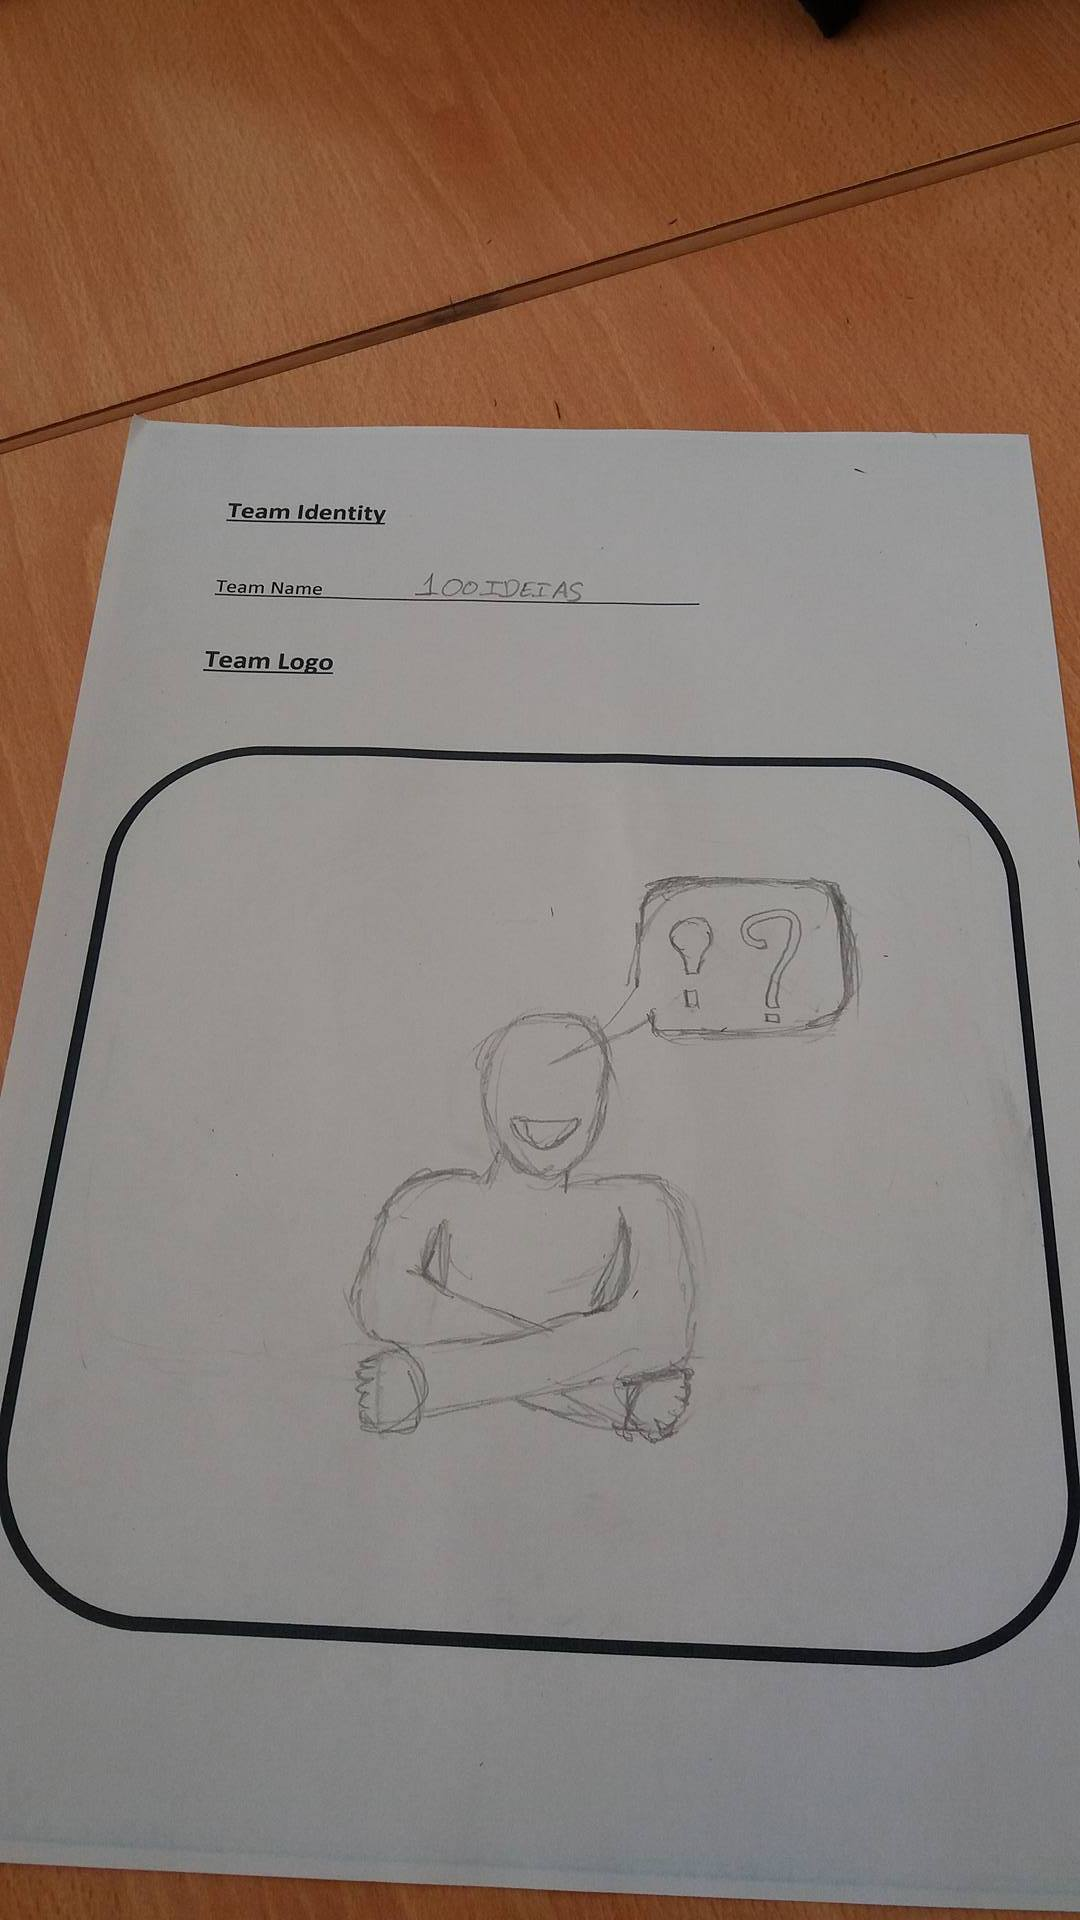
\includegraphics[scale=1.7]{logo.jpg}
\caption{The Universe}
\label{fig:univerise}
\end{figure}

\section{Conclusion}
``I always thought something was fundamentally wrong with the universe'' \citep{adams1995hitchhiker}

\bibliographystyle{plain}
\bibliography{references}
\end{document}
